\documentclass[dvipsnames, svgnames, x11names]{beamer}
\usepackage[UTF8, noindent]{ctexcap}  % 中文支持、无段前缩进

\usepackage{multicol}  % 双栏目录
\usepackage{setspace}  % 调整行距
\usepackage{listings}

% \usepackage{ctex}
\usepackage{tikz}
\usepackage{xcolor}

% 代码抄录的一系列设置
\lstset{
    basicstyle=\footnotesize\ttfamily, 
    flexiblecolumns, 
    numbers=left, 
    numbersep=5pt, 
    numberstyle=\tiny, 
    backgroundcolor=\color{white}, 
    frame=single, 
    breaklines=true, 
    showtabs=false, 
    showspaces=false, 
    showstringspaces=false, 
    keywordstyle=\color{teal}, 
    commentstyle=\color{blue}, 
    stringstyle=\color{red}, 
    numberstyle=\color{gray}, 
    tabsize=8, 
    breakatwhitespace=false, 
    postbreak=\mbox{\textcolor{violet}{$\hookrightarrow$}\space}
} % 代码抄录的一系列设置


\mode<presentation> {
	%set the slide theme
	% \usetheme{Frankfurt}
    \useoutertheme[footline=authorinstitutetitle,subsection=false]{smoothbars}
    \useinnertheme{circles}
	% \setbeamertemplate{caption}[numbered]
	% \setbeamercolor{footcolorleft}{fg=white, bg=black} 
	% \setbeamercolor{footcolorright}{parent=title}
	% \setbeamercolor{part title}{fg=white, bg=black}
	% \setbeamertemplate{footline}{
	% 	\hbox{%
	% 		\begin{beamercolorbox}[wd=.5\paperwidth,ht=2.6ex,dp=1ex,left,leftskip=2ex]{footcolorleft} 
	% 			\usebeamerfont{section in foot}CSUST BO 编译器的设计与实现
	% 		\end{beamercolorbox}%
	% 		\begin{beamercolorbox}[wd=.5\paperwidth,ht=2.6ex,dp=1ex,right,rightskip=2ex]{footcolorright} 
	% 			\usebeamerfont{section in foot}\insertframenumber\,/\,\inserttotalframenumber 
	% 		\end{beamercolorbox}}%
	% 	}
  \setbeamertemplate{footline} 
  {%
    \begin{beamercolorbox}[colsep=1.5pt]{upper separation line foot}
    \end{beamercolorbox}
    \begin{beamercolorbox}[ht=2.5ex,dp=1.125ex,%
      leftskip=.3cm,rightskip=.3cm plus1fil]{author in head/foot}%
      \leavevmode{\usebeamerfont{author in head/foot}\insertshortauthor}%
      \hfill%
      {\usebeamerfont{institute in head/foot}\usebeamercolor[fg]{institute in head/foot}\insertshortinstitute}%
    \end{beamercolorbox}%
    \begin{beamercolorbox}[ht=2.5ex,dp=1.125ex,%
      leftskip=.3cm,rightskip=.3cm plus1fil]{title in head/foot}%
      {\usebeamerfont{title in head/foot}\insertshorttitle}%
      \hfill%
      {\usebeamerfont{frame number}\usebeamercolor[fg]{frame number}\insertframenumber~/~\inserttotalframenumber}
    \end{beamercolorbox}%
    \begin{beamercolorbox}[colsep=1.5pt]{lower separation line foot}
    \end{beamercolorbox}
  }
	% \setbeamercovered{transparent}	
	\hypersetup{pdfpagemode=FullScreen}

    
% \xdefinecolor{csust_bg}{rgb}{0.03125,0.40625,0.70703125}  %RGB 8,104,181
% \xdefinecolor{csust_bg}{rgb}{0.046875, 0.390625, 0.625}  %RGB 12,100,160
\xdefinecolor{csust_bg}{rgb}{0.10546875, 0.19921875, 0.54296875}  %RGB 27,51,139
\setbeamercolor{footline}{bg=csust_bg}
\setbeamercolor{frametitle}{bg=csust_bg,fg=white}
\setbeamercolor{title}{bg=csust_bg}
\setbeamerfont{frametitle}{size=\large}
%\setbeamertemplate{navigation symbols}{}
% \setbeamertemplate{bibliography item}[text]
\setbeamertemplate{caption}[numbered]

\setbeamercolor{palette primary}{use=structure,fg=white,bg=structure.fg}
\setbeamercolor{palette secondary}{use=structure,fg=white,bg=structure.fg!75!black}
\setbeamercolor{palette tertiary}{use=structure,fg=white,bg=structure.fg!50!black}
\setbeamercolor{palette quaternary}{fg=white,bg=structure.fg!50!black}
%\setbeamercolor*{sidebar}{use=structure,bg=structure.fg}
\setbeamercolor{titlelike}{parent=palette primary}

%% try
\setbeamercolor{block title}{bg=csust_bg,fg=white}
\setbeamercolor*{block title example}{use={normal text,example text},bg=white,fg=csust_bg}
\setbeamercolor{fine separation line}{}
\setbeamercolor{item projected}{fg=white}
\setbeamercolor{palette sidebar primary}{use=normal text,fg=normal text.fg}
\setbeamercolor{palette sidebar quaternary}{use=structure,fg=structure.fg}
\setbeamercolor{palette sidebar secondary}{use=structure,fg=structure.fg}
\setbeamercolor{palette sidebar tertiary}{use=normal text,fg=normal text.fg}
%\setbeamercolor{palette sidebar quaternary}{fg=white}
\setbeamercolor{section in sidebar}{fg=brown}
\setbeamercolor{section in sidebar shaded}{fg=grey}
\setbeamercolor{separation line}{}
\setbeamercolor{sidebar}{bg=csust_bg}
\setbeamercolor{sidebar}{parent=palette primary}
\setbeamercolor{structure}{fg=csust_bg}
\setbeamercolor{subsection in sidebar}{fg=brown}
\setbeamercolor{subsection in sidebar shaded}{fg=grey}
    \AtBeginSection[]{
        \begin{frame}[plain]
            \tableofcontents[sectionstyle=show/shaded,subsectionstyle=show/shaded/hide,subsubsectionstyle=show/shaded/hide]
        \end{frame}
    }
    \AtBeginSubsection[]{
        \begin{frame}[plain]
            \tableofcontents[sectionstyle=show/shaded,subsectionstyle=show/shaded/hide,subsubsectionstyle=show/shaded/hide]
        \end{frame}
    }
} % end mode <presentation>

\title{BO 编译器的设计与实现}
\subtitle{The Design and Implementation of BO Compiler}
\author[周博]{\makebox[4em][s]{演讲人}:\makebox[4em][l]{周博}\\ 指导教师:项洁老师}
\institute[长沙理工大学计算机与通信工程学院]{长沙理工大学计算机与通信工程学院\\ 软件工程18-4班}
\date{2022年6月7日}
\titlegraphic{\includegraphics[width=3cm]{../figure/csust_logo.jpg}}
% \logo{\includegraphics{../figure/csust_logo.jpg}}

% \usetheme{PaloAlto}  % 幻灯片风格

\subject{编译原理}
\keywords{编译器、BO语言}

\begin{document}

\begin{frame}[plain]
    \titlepage
\end{frame}
%%%%%%%%%%%%%%%%%%%%%%%%%%%%%%%%%%%%%%%%%%%%%
% 各位老师好,我是软件 1804 班的周博,我的毕设课题是:BO 编译器的设计与实现。
% 
%%%%%%%%%%%%%%%%%%%%%%%%%%%%%%%%%%%%%%%%%%%%%

\begin{frame}[plain]
    \tableofcontents[sectionstyle=show,subsectionstyle=show/shaded/hide,subsubsectionstyle=show/shaded/hide]
	% \begin{spacing}{1.2}
	% 	\begin{multicols}{2}
	% 		{{\small \tableofcontents}}
	% 	\end{multicols}
	% \end{spacing}
\end{frame}
%%%%%%%%%%%%%%%%%%%%%%%%%%%%%%%%%%%%%%%%%%%%%
% 下面,我会先介绍本课题的主要研究对象和研究重点,
% 然后对 BO 编译器的各个模块的功能进行说明,
% 之后展示实现这个编译器用到的一些数据结构和关键技术,
% 最后总结这个版本的 BO 编译器的优缺点。
%%%%%%%%%%%%%%%%%%%%%%%%%%%%%%%%%%%%%%%%%%%%%

%%%%%%%%%%%%%%%%%%%%%%%%%%%%%%%%%%%%%%%%%%%%%
% 首先是课题介绍。
% BO 编译器,顾名思义,就是用来编译 BO 程序的编译器,因此我们先要知道 BO 程序的运行步骤。
% 
%%%%%%%%%%%%%%%%%%%%%%%%%%%%%%%%%%%%%%%%%%%%%
\section{课题介绍}
\subsection{BO 程序的运行步骤}
\begin{frame}
    \begin{minipage}{.4\linewidth}
    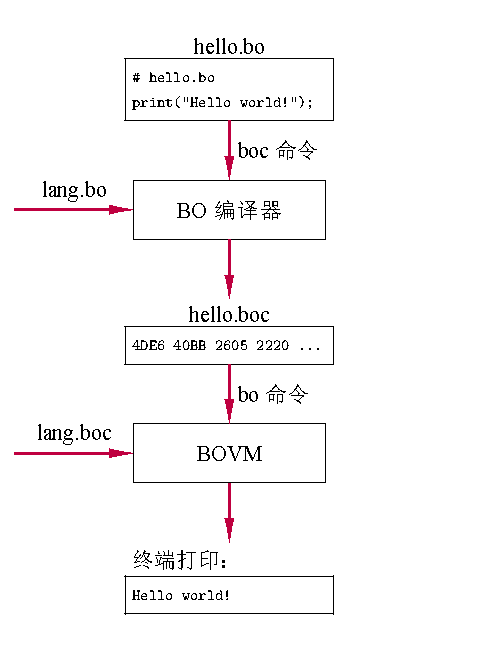
\includegraphics[height=\textheight]{../figure/compileProcess(1).pdf}
    \end{minipage}
    \quad\quad
    \begin{minipage}{.5\linewidth}
    \onslide<+-> BO(Binary Object) 语言是一种静态类型的编译型语言。
    \onslide<+-> BO 程序的运行步骤如下:
    \begin{itemize}[<+->]
        \item 将用 BO 语言写好的源代码以 \texttt{.bo} 格式保存。
        \item 使用 \alert{boc} 命令编译 \texttt{.bo} 格式文件,由BO编译器生成 \texttt{.boc} 格式的字节码文件。
        \item 使用 \alert{bo} 命令执行 \texttt{.boc} 格式的字节码文件,由BOVM虚拟机运行得到结果。
    \end{itemize}
    \end{minipage}
\end{frame}
%%%%%%%%%%%%%%%%%%%%%%%%%%%%%%%%%%%%%%%%%%%%%
% 我们可以结合左边这副图来理解 BO 程序的运行步骤。
% 这里写好了一个 BO 程序,并且保存在了 hello.bo 这个文件中,这个程序只有一行代码,用于输出 Hello world。BO 语言的单行注释以 # 号开头。
% 对这个文件使用 boc 命令之后,BO 编译器会对它进行一系列处理并输出 hello.boc 文件。 
% BO 编译器同时还会编译 hello.bo 中导入的外部文件,左边这个 lang.bo 文件是编译器自动导入的,里面包含 print 函数的定义。
% 由于 lang.bo 在上一次编译之后没有修改过,因此 BO 编译器没有重新为它生成 lang.boc 文件。
% BOC 文件中的前 4 个字节用于告诉虚拟机这是一个合法的 BOC 文件,接下来的四个字节指定文件要求的虚拟机版本号,再往后就是 BOVM 虚拟机运行所需的。
% 都是以小端方式存入的。
% 从 hello.boc 的二进制代码可以看出它期望的虚拟机版本号是 20220526 也就是 5月26号 的版本。
% 最后对 hello.boc 文件使用 bo 命令就能运行得到结果了。 BOVM 虚拟机在运行的时候也会导入外部的 boc 文件进行链接。
%%%%%%%%%%%%%%%%%%%%%%%%%%%%%%%%%%%%%%%%%%%%%

%%%%%%%%%%%%%%%%%%%%%%%%%%%%%%%%%%%%%%%%%%%%%
% 我的毕设课题是 BO 编译器的设计与实现。因此后面的内容主要是对 BO 编译器的介绍,对 BO 语言和 BOVM 虚拟机都不会有过多的介绍。
% 
%%%%%%%%%%%%%%%%%%%%%%%%%%%%%%%%%%%%%%%%%%%%%
\begin{frame}
    \begin{center}
        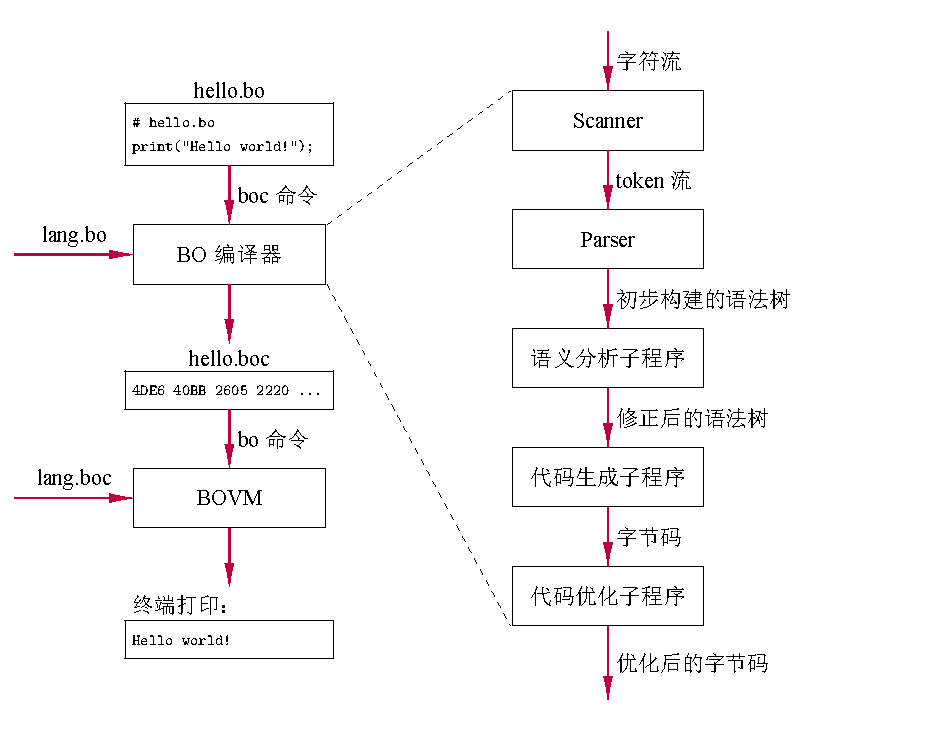
\includegraphics[height=\textheight]{../figure/compileProcess.pdf}
    \end{center}
\end{frame}
%%%%%%%%%%%%%%%%%%%%%%%%%%%%%%%%%%%%%%%%%%%%%
% 将图中的 BO编译器的盒子 进行展开,就变成了这样,BO 编译器的每一个流程就是一个功能模块,这也是后面要介绍的内容。
% 
%%%%%%%%%%%%%%%%%%%%%%%%%%%%%%%%%%%%%%%%%%%%%

\subsection{本课题的研究重点}
\begin{frame}
    \begin{minipage}{.5\linewidth}
    \onslide<+-> 本课题的研究重点在于如何实现一个能满足下列要求的BO编译器:
    \begin{itemize}[<+-| alert@+>]
        \item 正确编译 BO 源程序,生成 \texttt{.boc} 格式的字节码文件。
        \item 为存在错误的 BO 源程序报告尽可能准确的出错信息。
        \item 在编译阶段尽可能多地发现 BO 源程序的语义错误。
        \item 生成尽可能优化的字节码程序。
    \end{itemize}
    \end{minipage}
    \quad\quad
    \begin{minipage}{.4\linewidth}
    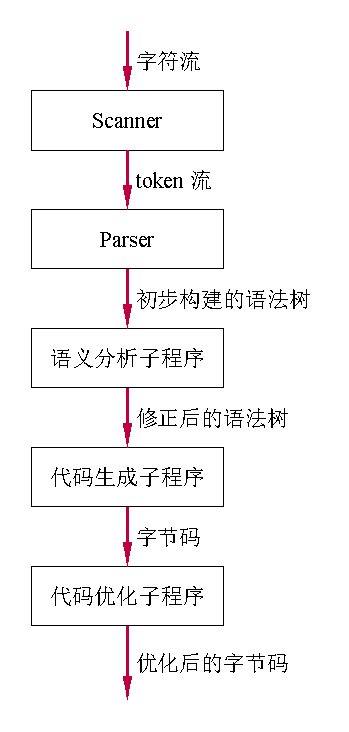
\includegraphics[height=\textheight]{../figure/compileProcess(2).pdf}
    \end{minipage}
    {\onslide<+->}
\end{frame}
%%%%%%%%%%%%%%%%%%%%%%%%%%%%%%%%%%%%%%%%%%%%%
% 本课题的重点就是实现这样一个编译器:能正确编译BO程序、提示出错信息、优化代码、生成 boc 文件。
% 
%%%%%%%%%%%%%%%%%%%%%%%%%%%%%%%%%%%%%%%%%%%%%
    
\section{系统功能模块}
\begin{frame}
    \begin{minipage}{.5\linewidth}
    \onslide<+-> BO 编译器具有如下功能:
    \begin{itemize}[<+->]
        \item 词法分析
        \item 语法分析
        \item 语义分析
        \item 代码生成
        \item 代码优化
    \end{itemize}
    \onslide<+-> 每个功能模块都会用到符号表和出错处理程序。
    \end{minipage}
    \quad\quad
    \onslide<1->
    \begin{minipage}{.4\linewidth}
    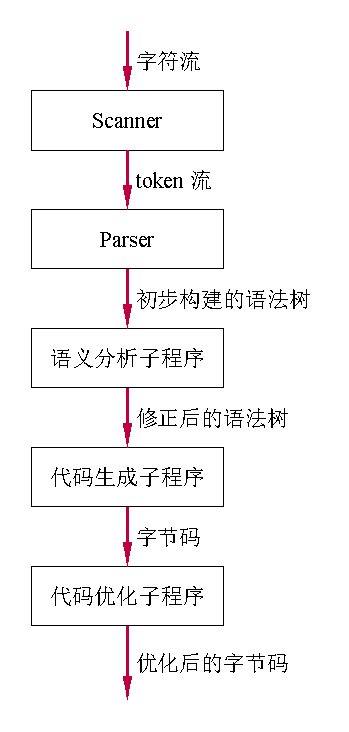
\includegraphics[height=\textheight]{../figure/compileProcess(2).pdf}
    \end{minipage}
\end{frame}
%%%%%%%%%%%%%%%%%%%%%%%%%%%%%%%%%%%%%%%%%%%%%
% BO 编译器的主要功能就是 词法分析、语法分析、语义分析、代码生成和代码优化,接下来我会逐个介绍这些模块。
% 每个功能模块都会用到符号表和出错处理程序。
% 
%%%%%%%%%%%%%%%%%%%%%%%%%%%%%%%%%%%%%%%%%%%%%

\subsection{词法分析}
\begin{frame}
    \begin{minipage}{.4\linewidth}
    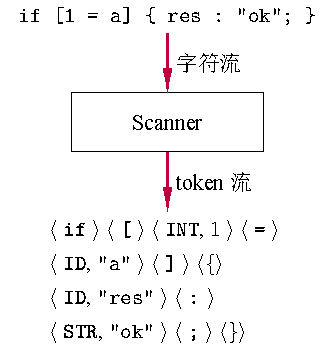
\includegraphics[width=\linewidth]{../figure/scanner.pdf}
    \end{minipage}
    \quad
    \begin{minipage}{.55\linewidth}
    \onslide<+->词法分析器(Scanner)的工作流程:
    \begin{itemize}[<+->]
        \item 从源文件中不断读入一个个字符。
        \item 将单个字符组合成一个个词素。
        \item 以词法单元(token)的形式返回给调用者。
    \end{itemize}
    \onslide<+->词法分析器发现\alert{非预期}的字符时会报告相应错误。
    %(如字符串环境中出现显示换行、代码环境中出现字符@等)
    \end{minipage}
\end{frame}
%%%%%%%%%%%%%%%%%%%%%%%%%%%%%%%%%%%%%%%%%%%%%
% 我们先来看词法分析器。
% Scanner 会依次对源程序中的每一个字符进行处理
% 剔除多余的空白字符,识别出词素,并以词法单元的形式返回给调用者
% 图中展示了 Scanner 对 if 子句进行分析并返回词法单元。
%%%%%%%%%%%%%%%%%%%%%%%%%%%%%%%%%%%%%%%%%%%%%

\subsection{语法分析}
\begin{frame}
    \begin{minipage}{.4\linewidth}
    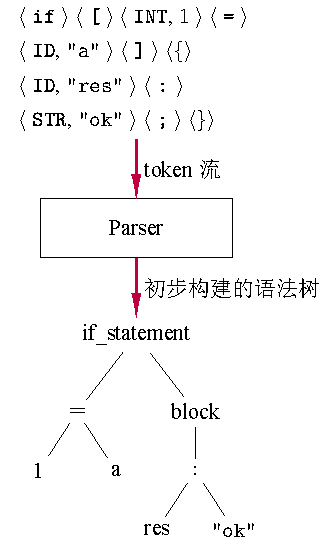
\includegraphics[width=\linewidth]{../figure/parser1.pdf}
    \end{minipage}
    \quad
    \begin{minipage}{.55\linewidth}
    \onslide<+->语法分析器(Scanner)的工作流程:
    \begin{itemize}[<+->]
        \item 调用词法分析器获取一个个词法单元。
        \item 不断移进词法单元并进行规约。
        \item 在规约的过程中初步构建一颗抽象语法树。
        \item 规约完成后得到的抽象语法树即为源程序的一个中间表示。
    \end{itemize}
    \onslide<+->语法分析器发现\alert{非预期}的词法单元时会报告相应错误。
    %(如非布尔表达式中出现 \texttt{\bfseries =} 等)
    \end{minipage}
\end{frame}

\begin{frame}
    语法分析器进行规约的过程,实际上是对语法分析树自底向上遍历的过程。
    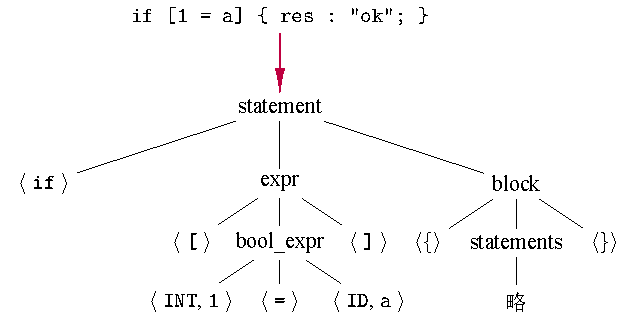
\includegraphics{../figure/parser2.pdf}
\end{frame}

\subsection{语义分析}
\begin{frame}
    \begin{minipage}{.4\linewidth}
    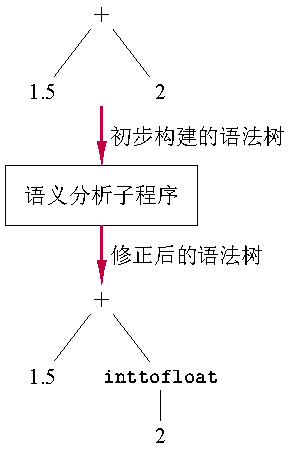
\includegraphics[width=\linewidth]{../figure/semantic.pdf}
    \end{minipage}
    \quad
    \begin{minipage}{.55\linewidth}
    \begin{itemize}[<+->]
        \item 语法分析阶段已经初步构建出了一颗抽象语法树。
        \item 语义分析阶段要做的就是遍历抽象语法树,进行类型检查、变量作用范围检查、以及类成员访问合法性检查。
        \item 一旦语义分析子程序发现语义问题,就会进行修正或者直接报错。
    \end{itemize}
    \end{minipage}
\end{frame}

\begin{frame}
    BO 语言将 $3>2>1$ 解释为 $3>2\&\&2>1$,因此需要在语法分析阶段进行修正。

    \vspace{\baselineskip}
    \begin{center}
    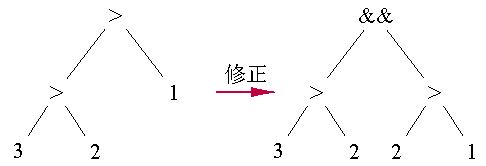
\includegraphics{../figure/semantic1.pdf}
    \end{center}
    
\end{frame}

\begin{frame}
    BO 语言不支持整数类型与布尔类型做算术运算。如果出现形如 $1+\texttt{\bfseries true}$ 的表达式,会在语义分析阶段发现表达式类型不匹配。

    \vspace{\baselineskip}
    \begin{center}
    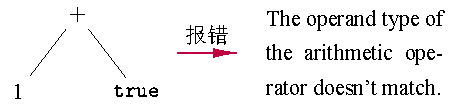
\includegraphics{../figure/semantic2.pdf}
    \end{center}
\end{frame}

\subsection{代码生成}
\begin{frame}
    \begin{minipage}{.4\linewidth}
    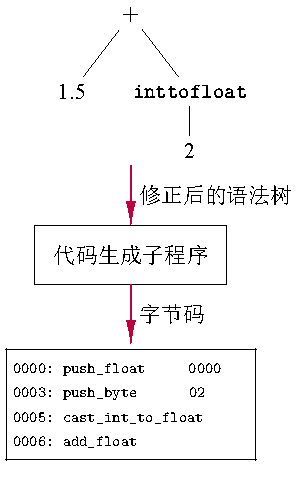
\includegraphics[width=\linewidth]{../figure/generator.pdf}
    \end{minipage}
    \quad
    \begin{minipage}{.55\linewidth}
    \begin{itemize}[<+->]
        \item 对修正后的语法树进行后序遍历,即可生成字节码。
        \item 一条\alert{字节码指令}由操作码和操作数组成。
        \item 字节码指令最多占 3 个字节,其中操作码固定占 1 个字节。
        \item 对于超过 2 个字节的操作数,BO 编译器会将其加入\alert{常量池},并通过索引访问。
    \end{itemize}
    \onslide<+->注:为方便演示、本幻灯片中的字节码均以\alert{助忆符}的形式呈现。
    \end{minipage}
\end{frame}

\begin{frame}
    为流程控制语句生成代码时,需要两次遍历,才能确定需要跳转的位置的地址。

    \vspace{\baselineskip}
    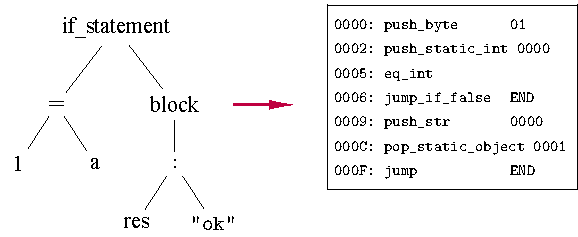
\includegraphics{../figure/generator1(1).pdf}
\end{frame}

\begin{frame}
    为流程控制语句生成代码时,需要两次遍历,才能确定需要跳转的位置的地址。

    \vspace{\baselineskip}
    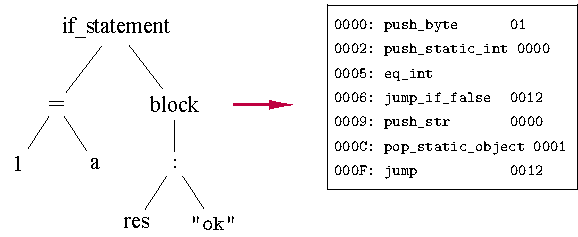
\includegraphics{../figure/generator1.pdf}
\end{frame}

\subsection{代码优化}
\begin{frame}
    \begin{minipage}{.4\linewidth}
    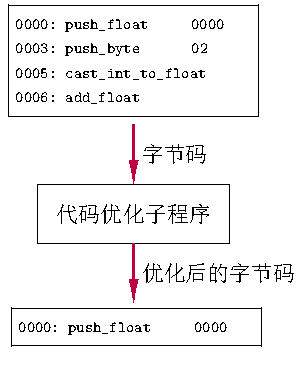
\includegraphics[width=\linewidth]{../figure/optimizer.pdf}
    \end{minipage}
    \quad
    \begin{minipage}{.55\linewidth}
    \onslide<+->BO 编译器会对生成的字节码进行简单的常量折叠和死码消除,
    \onslide<+->其中包括:
    \begin{itemize}[<+->]
        \item 计算字面量表达式。
        \item 消除条件为 false 的 if 和 while 语句,以及循环次数为 0 的 repeat 语句。
        \item 展开条件为 true 的 if 语句,以及循环次数为 1 的 repeat 语句。
        \item 对每一个代码块,消除 return、break 和 continue 之后的语句。
    \end{itemize}
    \end{minipage}
\end{frame}

\begin{frame}
    简单的常量折叠工作。

    \vspace{\baselineskip}
    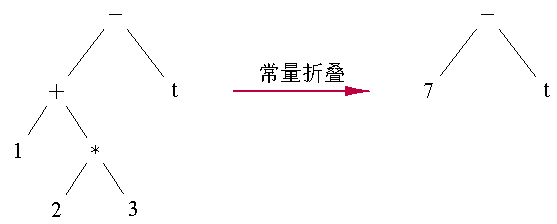
\includegraphics{../figure/optimizer1.pdf}
\end{frame}

\begin{frame}
    简单的常量折叠工作。

    \vspace{\baselineskip}
    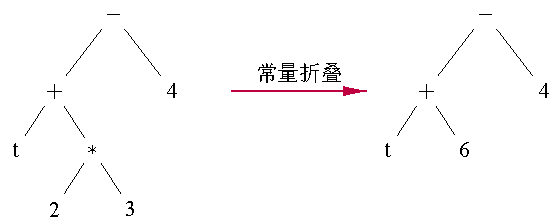
\includegraphics{../figure/optimizer2.pdf}
\end{frame}

\begin{frame}
    对 return 之后的语句直接消除。

    \vspace{\baselineskip}
    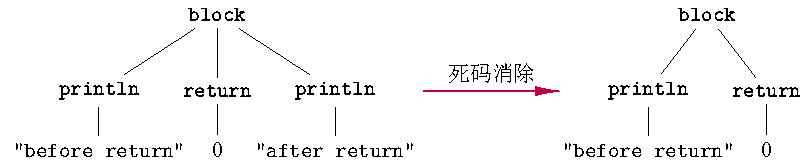
\includegraphics[width=\linewidth]{../figure/optimizer3.pdf}
\end{frame}

\begin{frame}
    对循环次数为 1 的 repeat 语句进行展开。

    \vspace{\baselineskip}
    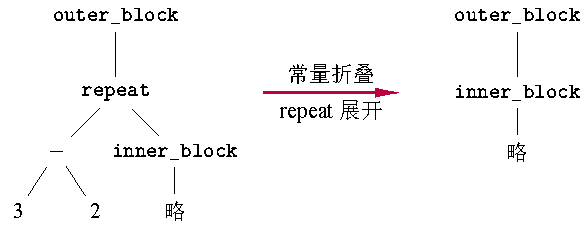
\includegraphics[width=\linewidth]{../figure/optimizer4.pdf}
\end{frame}


\section{BO 编译器的特点}

\subsection{BO 编译器的工作流程}
\begin{frame}
    \begin{itemize}[<+->]
        \item 在 BO 语言中,一个 \texttt{.bo} 文件就是一个包。
        \item 尽管 \texttt{boc} 命令只能指定一个文件名,但这个文件可能需要导入其他的包。
        \item 因此 BO 编译器也可能需要同时编译多个文件。
    \end{itemize}
\end{frame}

\begin{frame}
    \begin{center}
    \begin{minipage}{.4\linewidth}
        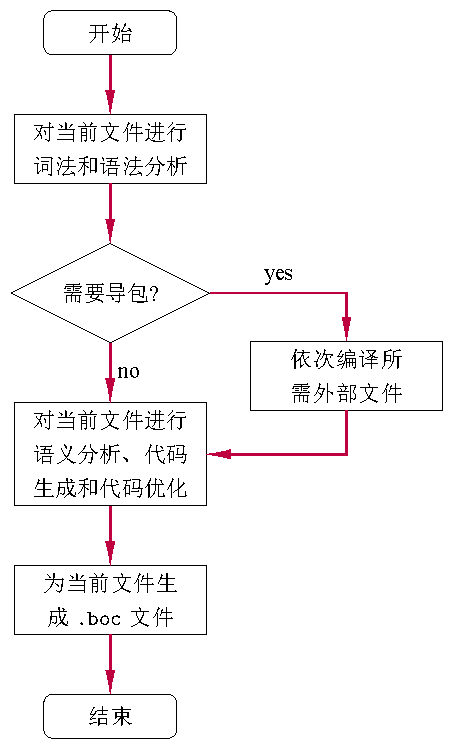
\includegraphics[height=\textheight]{../figure/flowChart.pdf}
    \end{minipage}
    \quad\quad
    \begin{minipage}{.45\linewidth}
        \begin{itemize}[<+->]
            \item 使用 BO 编译器编译多个文件的完整工作流程如图所示。
            \item 每编译一个文件,都会对其进行完整的词法和语法分析、导包、语义分析、代码生成和代码优化过程。
            \item 对于菱形导包的情况,BO 编译器可以保证每个文件仅被编译一次。
        \end{itemize}
    \end{minipage}
    \end{center}
\end{frame}

\subsection{BO 语言的特点}
\begin{frame}
    \begin{itemize}[<+->]
        \item BO 语言的语法是在设计与实现 BO 编译器的实践中逐渐形成和完善的。
        \item 因此可以认为能被 BO 编译器编译的语言就是 BO 语言。
        \item 也因此 BO 语言的特点实则也是 BO 编译器的特点。
    \end{itemize}
\end{frame}

\begin{frame}

    \begin{minipage}{.45\linewidth}
    \onslide<+-> 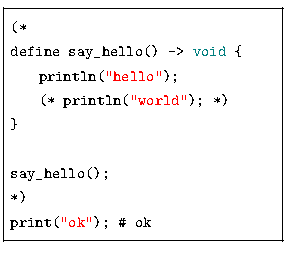
\includegraphics{../figure/characteristic4.pdf}
    \end{minipage}
    \begin{minipage}{.5\linewidth}
    \begin{itemize}[<+->]
        \item BO 语言支持\alert{嵌套}多行注释。
        \item 当用户想要注释一个带多行注释的函数时,嵌套多行注释的功能就显得十分有效。
    \end{itemize}
    \end{minipage}
\end{frame}

\begin{frame}

    \begin{minipage}{.45\linewidth}
    \onslide<+-> 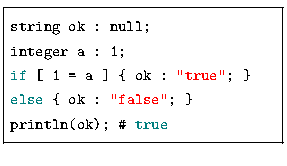
\includegraphics{../figure/characteristic3.pdf}
    \end{minipage}
    \begin{minipage}{.5\linewidth}
    \begin{itemize}[<+->]
        \item BO 语言使用 \texttt{:} 作为赋值符号,将 \texttt{=} 留作普通的相等符号。
        \item 实践证明这种符号表示方法更加符合人的直觉,也更容易被初学者接受。
        \item 然而为了避免使用主流语言的程序员误将 \texttt{=} 符号用于赋值,BO 语言规定布尔表达式必须用 \texttt{[]} 括起来。这一点也可能带来额外的不便。
    \end{itemize}
    \end{minipage}
\end{frame}

\begin{frame}
    不同于 C++ 和 Java, BO 语言将表达式
    \[
        \text{a} > \text{b} > \text{c} > \text{d}
    \]
    解释为
    \[
        \text{a} > \text{b} \land \text{b} > \text{c} \land \text{c} > \text{d}
    \]
    这一点更符合数学上的直觉。
\end{frame}

\begin{frame}

    \onslide<+-> BO 语言提供 repeat 语句,可以指定重复次数。

    \begin{center}
    \onslide<+-> 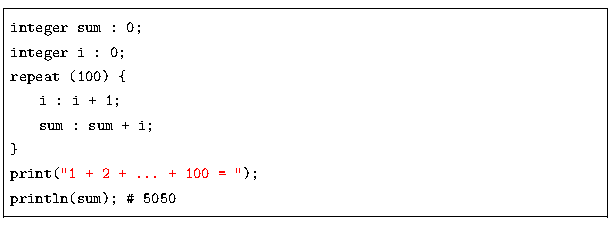
\includegraphics{../figure/characteristic1.pdf}
    \end{center}

    \onslide<+-> 这也是推荐初学者使用的循环语句,因为初学者使用 while 语句时容易造成死循环。
\end{frame}

\begin{frame}
    \onslide<+-> BO 语言的构造函数使用 constructor 关键字声明。

    \begin{center}
    \onslide<+-> 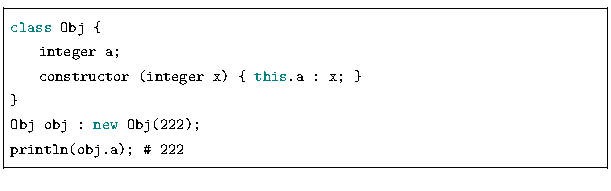
\includegraphics{../figure/characteristic2.pdf}
    \end{center}

    \onslide<+-> 虽然很多主流语言使用类名作为构造函数名,但这确实不是一个好的规则,也不符合程序员的直觉。
\end{frame}


% \section{数据结构设计}
% \subsection{词法分析器和语法分析器的设计}
% \begin{frame}
%     \onslide<1>{第一步}

%     \onslide<2->{第二步}

%     \onslide<1,3>{第1,3步}
% \end{frame}

% \subsection{符号表的设计}
% \begin{frame}
% \end{frame}

\section{关键技术}

\subsection*{}
\begin{frame}
    \onslide<+-> BO 编译器的开发平台及开发工具如下:
    \begin{itemize}[<+->]
        \item Ubuntu 20.04.3
        \item Scanner 生成器 Flex 2.6.4
        \item Parser 生成器 Bison 3.5.1
        \item 采用 C++ 20 语言开发
        \item C++ 开发环境 CLion 2020.2.1
    \end{itemize}
    \onslide<+-> 下面将对 Flex 与 Bison 做进一步介绍。
\end{frame}

\subsection{Flex}
\begin{frame}{Flex(Fast LEXical analyzer generator)}
    \begin{itemize}[<+->]
        \item 是一个词法分析器的自动生成工具。
        \item 封装了基于词法规则构造有限自动机的过程。
        \item 支持使用正则表达式描述语法规则。
    \end{itemize}

    \vspace{\baselineskip}
    \onslide<+-> 在 Flex 的输入文件中指定 BO 语言的词法规则,和识别到对应词素时的动作,即可生成能够识别相应规则的词法分析器。
    
    \vspace{\baselineskip}
    \onslide<+-> 例:通过指定下列规则和对应的动作即可使词法分析器具有识别 BO 语言标识符并返回 token 的功能。

    \begin{center}
        \onslide<+->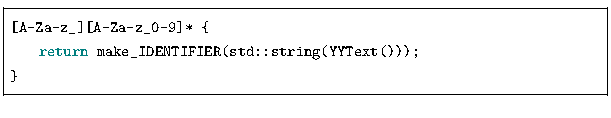
\includegraphics{../figure/flex1.pdf}
    \end{center}
\end{frame}

\begin{frame}{Flex(Fast LEXical analyzer generator)}
    \onslide<+->BO 语言嵌套多行注释的功能可通过下列规则和动作实现。
    
    \begin{center}
        \onslide<+->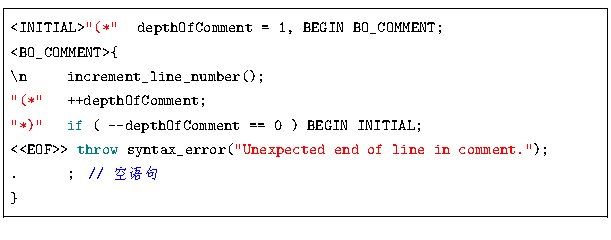
\includegraphics{../figure/flex2.pdf}
    \end{center}

    \onslide<+->其中变量 \texttt{depthOfComment} 记录嵌套的深度。
\end{frame}

\subsection{Bison}
\begin{frame}{Bison}
    \begin{itemize}[<+->]
        \item 是一个语法分析器的自动生成工具。
        \item 封装了基于语法规则构造 LR 分析器的过程。
        \item 使用类 BNF 范式描述语法规则。
    \end{itemize}

    \vspace{\baselineskip}
    \onslide<+-> 在 Bison 的输入文件中指定 BO 语言的语法规则,和识别到对应产生式时的动作,即可生成能够识别相应规则的语法分析器。
    
    \vspace{\baselineskip}
    \onslide<+-> 例:通过指定下列规则和对应的语义动作即可使词法分析器具有识别 BO 语言中 repeat 语句的功能。

    \begin{center}
        \onslide<+->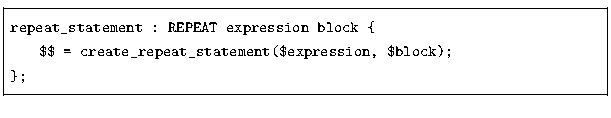
\includegraphics{../figure/bison1.pdf}
    \end{center}
\end{frame}

% \subsection{抽象语法树}
% \begin{frame}
% \end{frame}

\section{结语}
\subsection{BO 编译器的不足}
\begin{frame}
    \onslide<+-> BO 编译器的不足:
    
    \begin{itemize}[<+->]
        \item BO 语言缺乏丰富的标准库。
        \item BO 语言不支持闭包、多线程等当代程序设计语言必备的特性。
        \item BO 编译器加载程序导入的包的过程还有待优化。
    \end{itemize}

    \onslide<+-> 因此 BO 语言和 BO 编译器距离真正的实践还要很长的路要走。
\end{frame}

\subsection{BO 编译器的未来}
\begin{frame}
    \onslide<+->BO 语言要想在当代数百种程序设计语言中占有一席之地,就必须:

    \begin{itemize}[<+->]
        \item 最大限度地考虑用户的需求。
        \item 尽可能从其它语言中汲取精华、摒弃糟粕。
        \item 扩充标准库以达到使用标准。
    \end{itemize}
\end{frame}

\begin{frame}[plain]
    \begin{center}
        {\Huge Thanks!}
    \end{center}
\end{frame}

\end{document}